De la misma forma que el punto anterior, es de esperarse que la fuente tenga un valor mínimo de tensión de entrada, a partir del cual empieza a regular la salida, para valores menores de tensión que este valor mínimo, la corriente de salida será solo limitada a algún valor menor al esperado, y como puede verse en la figura~\figref{fig:fig_p19_io_vs_vi}, el crecimiento de la salida es prácticamente lineal, salvo que se produce un pico de corriente alrededor de los $3 V$ de entrada, que es limitado por la acción de $Q_{15}$, a ese valor de tensión de entrada el lazo de corriente seguramente no actúa de ninguna forma para limitar la corriente de salida. Tomando que la salida está regulando al llegar a aproximadamente al $1 \%$ de la corriente regulada esperada a la salida, $2.05 A$, el valor de tensión de entrada mínimo para salida regulada es de $12.19 V$, valor muy cercano al del punto anterior. También puede observarse que para tensiones muy pequeñas a la entrada, aproximadamente $1.8 V$, la tensión a la salida es prácticamente $0 A$, esto se explica por la misma razón que en el punto anterior.

\vfill

\clearpage

\begin{figure}[H] %htb
\begin{center}
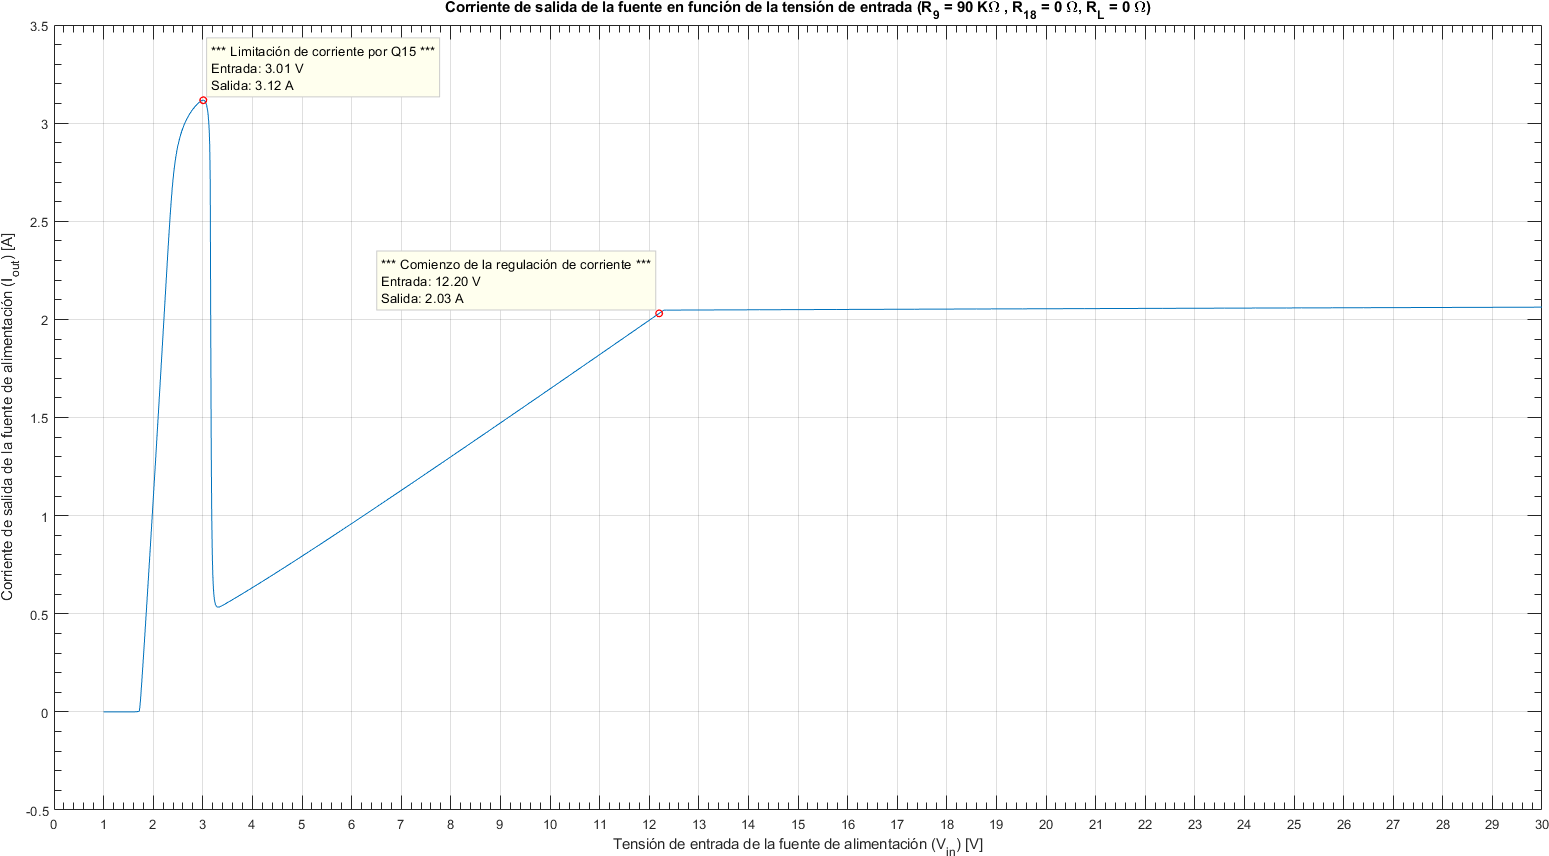
\includegraphics[width=1.2 \textwidth, angle=90]{./img/preguntas/p19.png}
\caption{\label{fig:fig_p19_io_vs_vi}\footnotesize{Tensión de salida vs tensión de entrada.}}
\end{center}
\end{figure}

\clearpage